\chapter {Analyzer}
\label{chap:analyzer}

The analyzer's role is to provide a facade over objects and methods to create a simple interface for processing (analyzing) a single HLASM source file. The output of the analysis is data for the LSP server.

\sectionSrc{Overview}
{parser\_library/src/analyzer.h}

The analyzer is composed of several sub-components, all required to properly process the file (see \cref{fig06:analyzer}). 
\begin{itemize}
	\item \emph{LSP data collector} collects and retrieves all LSP information created while processing the file.
	\item \emph{HLASM context tables} hold information about the context of the processed HLASM source code.
	\item The analyzer contains several \emph{Lexer - Parser sub-components} to simplify the processing interface and ease the use of this component. They are needed to create parser
	\item \emph{Processing manager} executes the main loop where the file is processed.
\end{itemize}

\begin{figure}
	\centering
	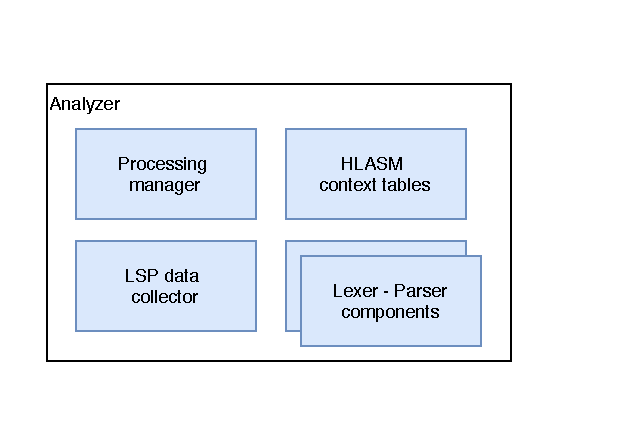
\includegraphics[width=\textwidth / 2]{img/analyzer_arch}
	\caption{The composition of the analyzer component}
	\label{fig06:analyzer}
\end{figure}

LSP data collector is required by Lexer-Parser sub-components. They are composed into the parser object required by processing manager. HLASM context tables are used by the manager and the sub-components as well. 

Presence of all this components together is needed for analyzer's method \TT{analyze}. It processes a provided file and fills LSP data collector from which LSP information can be further retrieved.  

\subsection{Construction}

In order to parse a HLASM file, the analyzer is constructed with the following parameters:
\begin{itemize}
	\item \emph{Name and content of the file}
	\item \emph{Parse library provider} -- an object responsible for resolving source file dependencies. The dependencies are only discovered during the analysis, so it is not possible to provide the files beforehand.
	\item \emph{Processing tracer} (see \cref{macro_tracer}).
\end{itemize}

When this constructor is used, the analyzer creates HLASM context tables and processes the provided source as an open-code. We say that the analyzer has \emph{owner semantics}. 
 
The analyzer provides \emph{reference semantics} as well. The provided source is not treated as an open-code, rather as an external file dependency. The constructor of an analyzer with reference semantics adds the following two parameters to the previous one:
\begin{itemize}
	\item \emph{HLASM context tables reference} --- belonging to the owning open-code analyzer.
	\item \emph{Library data} --- states how the dependency file should be treated (see \cref{lab06:lib_data}).
\end{itemize}

This constructor is called within open-code analyzer by its sub-components when they use the \emph{Parse library provider}.

\vspace{0.5cm}

To sum up, after the analyzer is constructed, it analyzes the provided source file. As a result, it updates HLASM context tables and provides a list of diagnostics linked to the file, highlighting, list of symbol definitions, etc.
